\documentclass[12pt]{exam}

\usepackage{fullpage, amsmath, amssymb, amsthm, graphicx}

\renewcommand{\partshook}{\setlength\itemsep{1em}}
\newcommand{\disp}{\displaystyle}
\newcommand{\CC}{\mathbb{C}}
\newcommand{\RR}{\mathbb{R}}
\renewcommand{\Re}{\operatorname{Re}}
\renewcommand{\Im}{\operatorname{Im}}
\DeclareMathOperator{\Log}{Log}
\DeclareMathOperator{\Arg}{Arg}
\DeclareMathOperator{\sign}{sign}
\begin{document}

\section*{MATH 307 --- Quiz \#1 }

\emph{Instructions:} You have 50 minutes to solve all three multipart problems.
All answers should be exact -- no decimal approximations.
No calculators, notes, or other aids.
Hand in only your solution booklet. 
There are 21 points available, plus 1 bonus point, but I'll record the grade out of 20.

\begin{questions}
    \setlength\itemsep{1.25em}
    \setlength\parskip{1em}

    \question\hfill

    \begin{parts}
        \part[2] Compute $|z|^2$, where $z=\dfrac{5i}{(1-i)(2-i)(3-i)}$.
        \begin{solution}
            \[
                \bar z z = |z|^2 = \frac{|5i|^2}{|1-i|^2|2-i|^2|3-i|^2} = \frac{25}{2\cdot5\cdot10}=\frac14
            \]
        \end{solution}

        \part[2] Express $\Log\left(\dfrac14 - \dfrac14i\right)$ in the form $x+iy$.
            Here, $\Log$ denotes the \textbf{principal branch} of the logarithm.

            \begin{solution}
                \begin{align*}
                    \Log\left(\dfrac14 - \dfrac14i\right) &= \log\left|\dfrac14 - \dfrac14i\right| + i\Arg\left(\dfrac14 - \dfrac14i\right)\\
                    &= \log\sqrt{\dfrac1{4^2} + \dfrac1{4^2}} + i\left(-\frac\pi4\right)\\
                    &= -\frac52\log2 - i\frac{\pi}4
                \end{align*}
            \end{solution}

        \part[2] Express $z=(\sqrt3-i)^6$ in the form $re^{i\theta}$.
       \begin{solution}
        Notice that $\sqrt3 - i = 2e^{-i\pi/6}$. Therefore,
        \[
            z = (\sqrt3 - i)^6 = (2e^{-i\pi/6})^6  = 2^6e^{-6i\pi/6} = 64e^{-i\pi}.
        \]
       \end{solution}
        
        \part[2] Let $w=e^{\bar{z}^2/2}$. Express $\Re(w)$ and $\Im(w)$ in terms of $x=\Re(z)$ and $y=\Im(z)$.
        \begin{solution} We compute:
        \begin{align*}
            e^{\bar z^2/2} &= e^{(x-iy)^2/2}\\
            &= e^{(x^2 - y^2 - 2xyi)/2}\\
            &=e^{(x^2+y^2)/2}e^{-xyi}\\
            &= e^{(x^2+y^2)/2}\big(\cos(-xy) + i\sin(-xy)\big)\\
            &= e^{(x^2+y^2)/2}\cos(xy) - ie^{(x^2+y^2)/2}\sin(xy).
        \end{align*}
        Thus,
        \[
            \Re(w) = e^{(x^2+y^2)/2}\cos(xy)\quad\text{and}\quad
            \Im(w) = e^{(x^2+y^2)/2}\sin(xy).
        \]

        \end{solution}

       

    \part[2] Find all values of $(-8i)^{1/3}$. Express them in the form $x+iy$.
    \begin{solution}
        \begin{align*}
            (-8i)^{1/3} = e^{\frac13\log(-8i)} &=e^{1/3(\log|-8i| + i\arg (-8i)}\\
            &=e^{\frac13\log 8 + \frac i3(-\frac\pi2 + 2k\pi)}\\
            &=e^2e^{i(-\frac\pi6 + \frac{k\pi}3)}\\
            &=e^2\cos\left(-\frac\pi6 + \frac{k\pi}3\right)+ ie^2\sin\left(-\frac\pi6 + \frac{k\pi}3\right),\quad k\in\mathbb{Z}.
        \end{align*}
    \end{solution}

    \end{parts}

    

    

    \question
    Sketch the sets in the complex plane, each on its own set of axes.
    Label points, radii, angles, etc. so that your meaning is unambiguous.
    \begin{parts}
        \part[2]
        $A = \{z : |z|<|z+1|\}$
        \part[2]
        $\displaystyle{B=\left\{z=re^{i\theta} : 1\leq r\leq2\;\;\text{and}\; -\frac\pi3\leq\theta \leq \frac\pi3\right\}}$

        \begin{solution}
    
            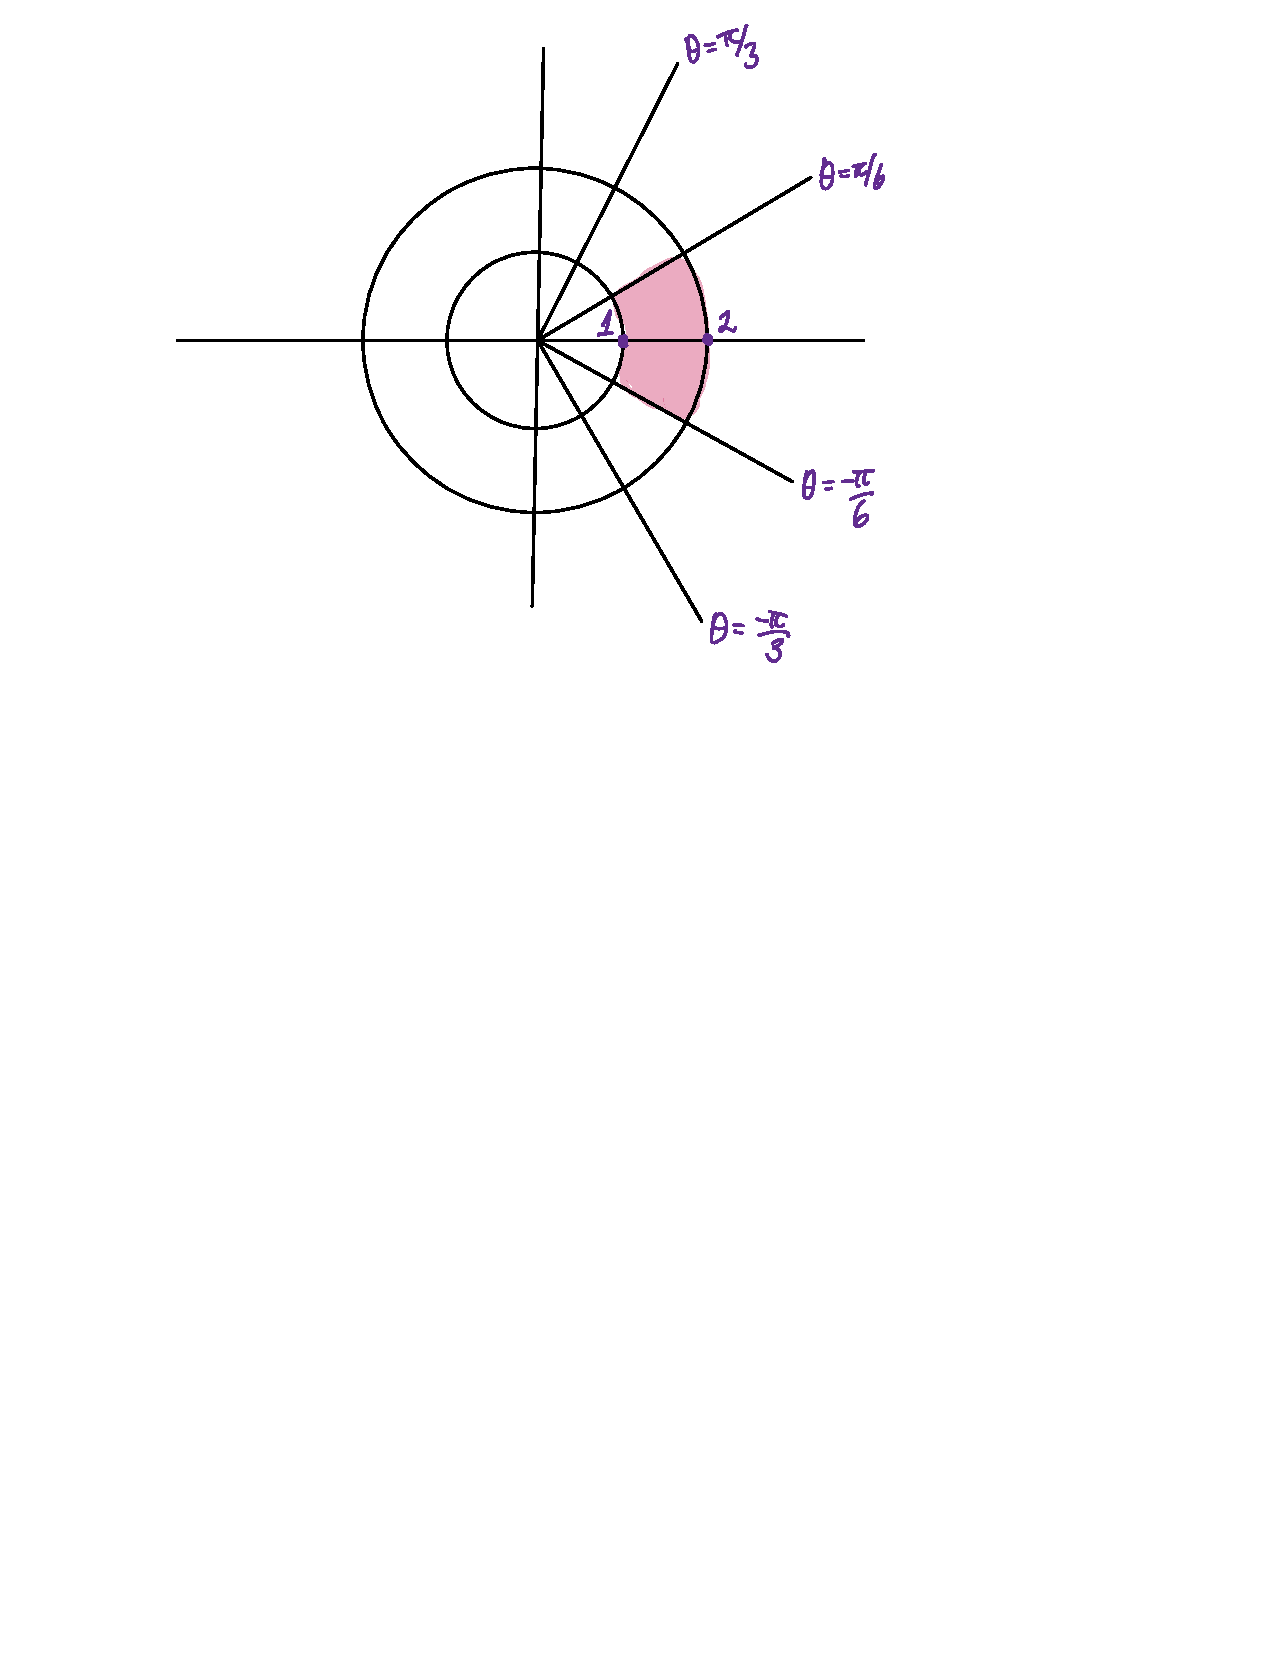
\includegraphics[scale=1]{a.pdf}
        \end{solution}

        \part[2]
        $\displaystyle{C=\{e^{i\pi/6}z^2 : z\in B\}}$
        \begin{solution}

            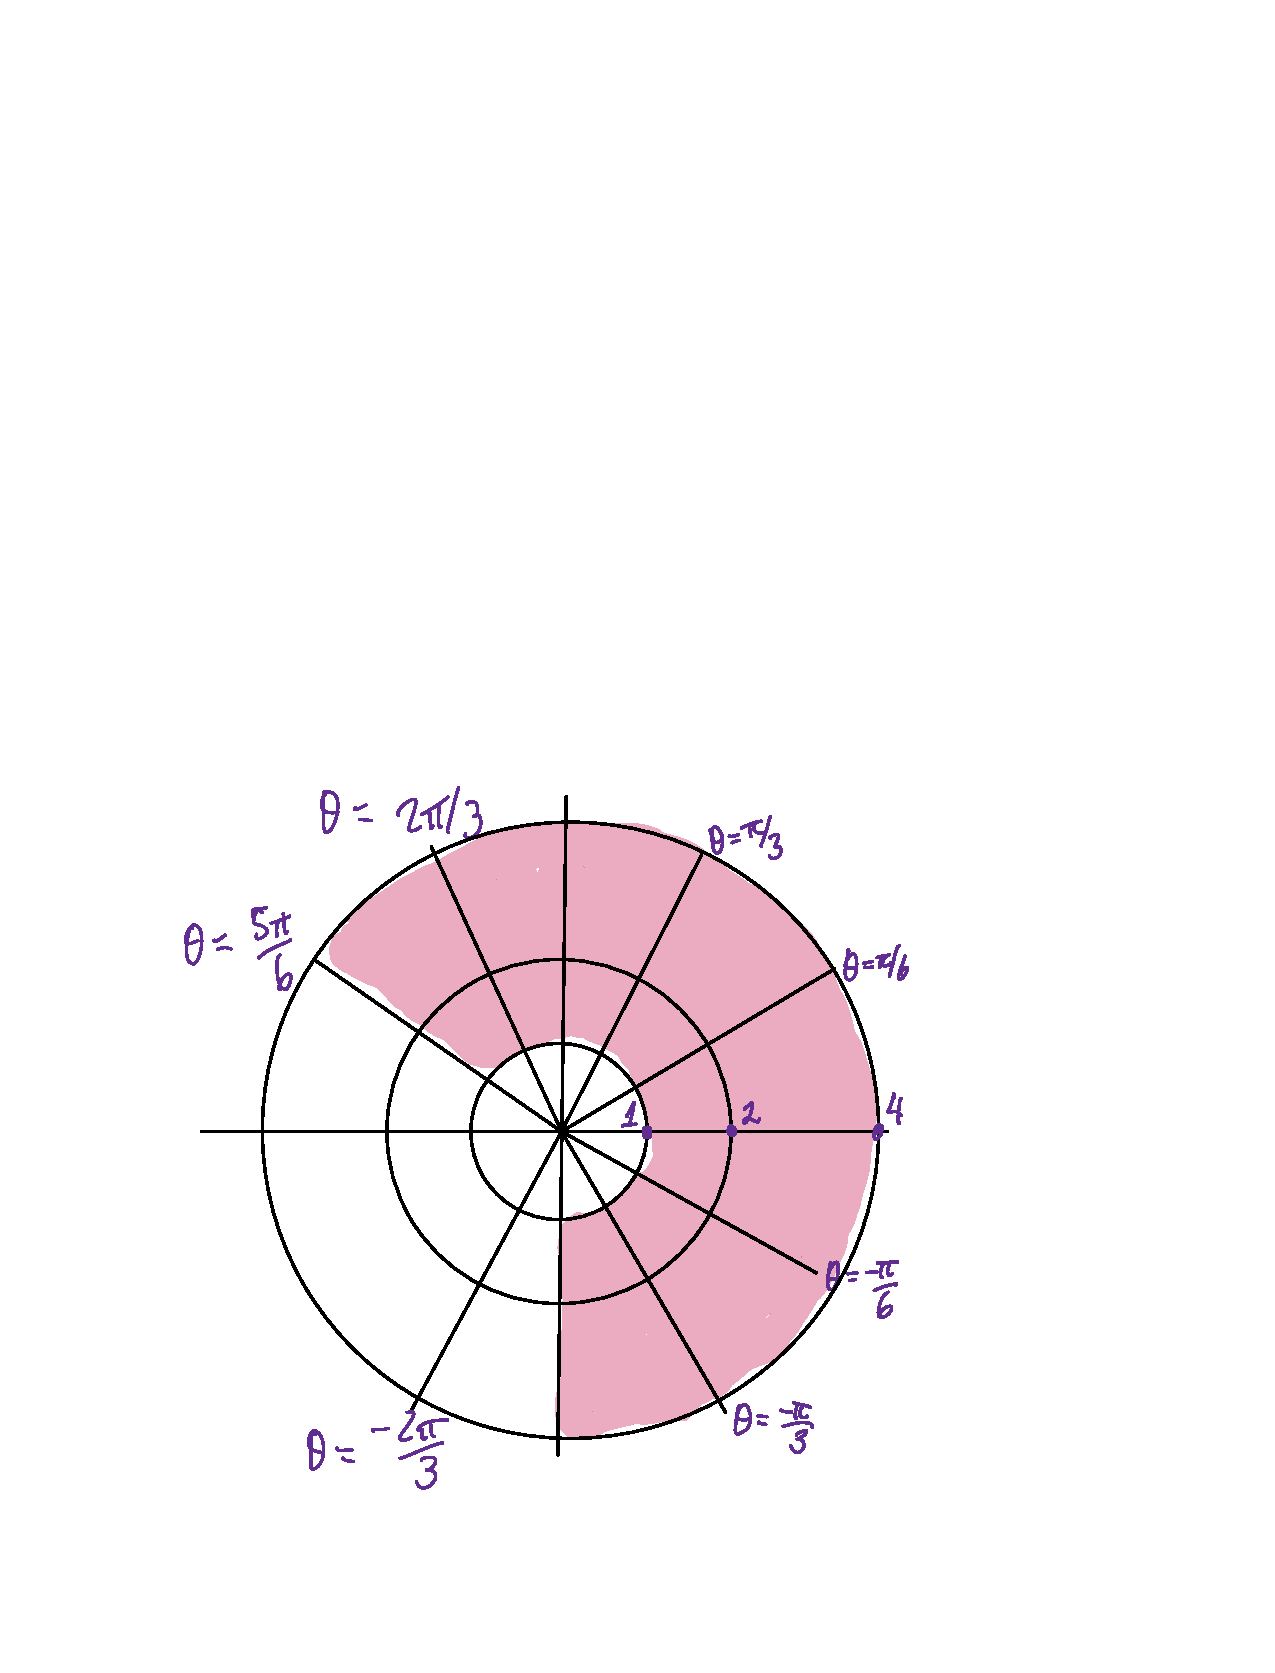
\includegraphics[scale=0.7]{b.pdf}
        \end{solution}

        \part[1] \fbox{ $\star\star$ \textsc{Bonus} $\star\star$ }
        $\displaystyle{D=\{z : z^2\in B\}}$
        \fbox{$\star\star$\textsc{Bonus}$\star\star$}
        \begin{solution}

            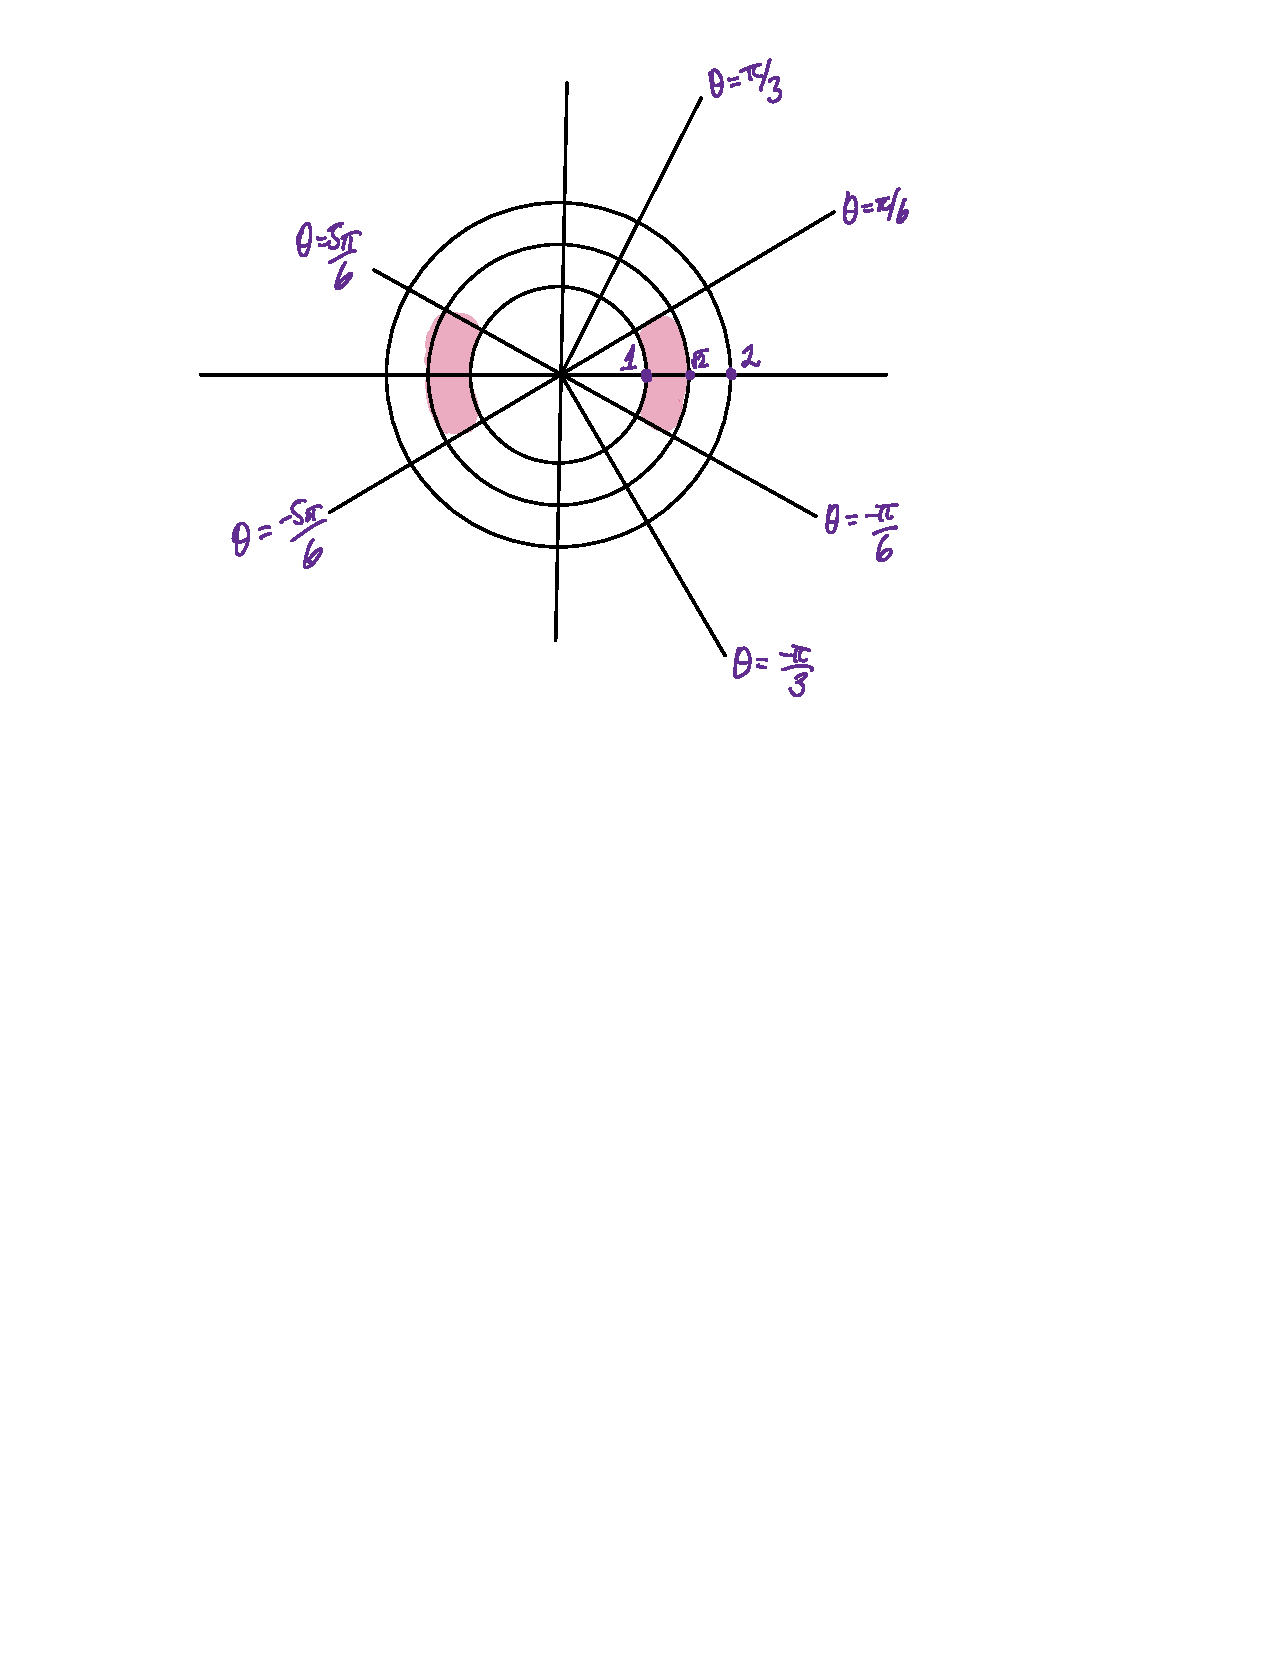
\includegraphics[scale=0.7]{c.pdf}
        \end{solution}
    \end{parts}
        
        
        
    \question[5]
    Let $\sqrt\cdot$ be the branch of the square root defined by
    \[
        \sqrt{re^{i\theta}} = \sqrt r\,e^{i\theta/2}\qquad\text{for}\qquad \theta\in [\pi, 3\pi).
    \]
    For which $z$ does $\sqrt{z^2}=z$ hold?
    
    Hint: Write $z=re^{i\psi}$ with $\psi\in[-\frac\pi2,3\pi)$. When computing $z^2$, consider the cases $\psi\in[-\frac\pi2,\frac\pi2)$ and $\psi\in[\frac\pi2,\frac{3\pi}2)$ separately.
    In each case, identify a $k$ such that $2\psi + 2\pi k$ belongs to $[\pi, 3\pi)$.

    \begin{solution}
        Suppose $\psi\in[-\frac\pi2,\frac\pi2)$.
        Then $2\psi\in[-\pi, \pi)$, so $\theta := \psi + 2\pi\in [\pi, 3\pi)$ and
        \[
            \sqrt{z^2} = \sqrt{r^2e^{i(2\psi)}} = \sqrt{r^2e^{i(2\psi+2\pi)}}=re^{i(\psi + \pi)}=re^{i\psi}e^{i\pi}=-z.
        \]
        If, on the other handm, $\psi\in[\frac\pi2,\frac{3\pi}2)$, then $2\psi\in [\pi, \frac{3\pi}2)$ and
        \[
            \sqrt{z^2} = \sqrt{r^2e^{i(2\psi)}} =re^{i(\psi + \pi)}=re^{i\psi}=z.
        \]
        Thus, $\sqrt{z^2}=z$ when $\psi\in [\frac\pi2,\frac{3\pi}2)$, i.e., when $\Re(z)<0$ or when $\Re(z)=0$ and $\Im(z)\geq 0$.
    \end{solution}
\end{questions}
\end{document}